% -*- coding: UTF-8; -*-
\documentclass[11pt,onecolumn]{article}
%Pour langue et caract�res sp�ciaux
\usepackage[french]{babel} 
\usepackage[T1]{fontenc}
\usepackage{lmodern}
\usepackage[latin1]{inputenc}

\usepackage[top=2cm, bottom=2cm, left=2cm, right=2cm, columnsep=20pt]{geometry}   %Pour ajuster les marges
\usepackage{graphicx}      %pour inclure des graphiques
\usepackage{url}           %Pour inclure des adresse web
\usepackage{verbatim}      %pour inclure les codes en annexe, on utilisera la commande verbatim
\usepackage{amsmath}
\DeclareMathOperator{\Tr}{Tr}
\usepackage{cancel}
\usepackage{color}
\usepackage{mathrsfs}
\usepackage{amssymb}
\usepackage{mathtools}
\usepackage{xfrac}
\usepackage{float}
\usepackage{wrapfig}
\usepackage{subcaption}
\usepackage{listings}
\lstset{
basicstyle=\small\ttfamily,
columns=flexible,
breaklines=true
}

\renewcommand{\baselinestretch}{1.5} 

\begin{document}

%Page titre
\begin{titlepage}
\center

\vspace*{2cm}

\textsc{\LARGE Universit� de Montr�al}\\[1cm] 
\textsc{\Large IFT6269 - Probabilistic Graphical Models}\\[1.5cm] 

\rule{\linewidth}{0.5mm} \\[0.5cm]
{\LARGE \bfseries Homework 2} \\[0.2cm] % Titre page titre
\rule{\linewidth}{0.5mm} \\[3cm]

\large by: \\*
Patrice B�chard\\*
20019173\\[8cm] 


{\large \today}\\[3cm]

\vfill
\end{titlepage}

\section{Generative model (Fisher LDA)}\label{sec:fisher_lda}

\begin{description}

 \item[(a)] Given $D = \left\{ (x_1,y_1), (x_2,y_2), \dots, (x_N,y_N) \right\}$ such that $ x_i \in \mathbb{R}^2$, $y_i \in \{0,1\}$. The data are assumed to be Gaussians with different means for different classes but with the same covariance matrix : 

\begin{equation*}
Y \sim \text{Bernoulli}(\Pi)
\qquad
X \mid Y=j \sim \mathcal{N}(\mu_j, \Sigma)
\end{equation*}

(We will use $\Pi$ instead of the more common $\pi$ to avoid confusion with the constant $\pi$ present in the gaussian distribution) We suppose that the data is \textit{iid}, which gives us :

\begin{equation*}
P(D) = \prod_{i=1}^{N} p(x_i,y_i)
\end{equation*}

We take the log-likelihood:

\begin{align} \label{eq:lda}
\log \prod_{i=1}^{N} p(x_i,y_i) & = \sum_{i=1}^{N} \log p(x_i,y_i) \nonumber \\
					& = \sum_{i=1}^{N} \log \left\{\left[ \Pi \mathcal{N}(x_i ; \mu_1, \Sigma)\right]^{y_i}\left[ (1-\Pi) \mathcal{N}(x_i; \mu_0,\Sigma)\right]^{1-y_i}\right\} \nonumber \\
					& = \sum_{i=1}^{N} \left\{ y_i \log \Pi + y_i \log \mathcal{N}(x_i; \mu_1,\Sigma) + (1-y_i) \log(1-\Pi) + (1-y_i)\log \mathcal{N}(x_i; \mu_0, \Sigma)  \right\} \nonumber \\
					& = \sum_{i=1}^{N} \left\{ y_i \log \Pi - \frac{2 y_i}{2}\log 2\pi -\frac{y_i}{2} \log |\Sigma| - \frac{y_i}{2} (x_i - \mu_1)^T \Sigma^{-1} (x_i - \mu_1) + (1-y_i) \log (1-\Pi) \right. \nonumber \\ 
				 	& \qquad \qquad - \left. \frac{2(1-y_i)}{2} \log 2\pi -\frac{1-y_i}{2} \log |\Sigma | - \frac{1-y_i}{2} (x_i-\mu_0)^T \Sigma^{-1} (x_i-\mu_0) \right\}
\end{align}

We first try to find $\Pi$ by deriving equation (\ref{eq:lda}) with respect to $\Pi$ and setting the equation equal to 0:

\begin{align*}
\frac{\partial}{\partial \Pi} (1) = \sum_{i=1}^{N} \left( \frac{y_i}{\Pi} - \frac{1-y_i}{1-\Pi} \right)  = 0
\end{align*}
\begin{align*}
\sum_{i=1}^{N} \frac{y_i}{\Pi}  &= \sum_{i=1}^{N} \frac{1-y_i}{1-\Pi} \\
\frac{1-\Pi}{\Pi} &= \frac{\sum_{i=1}^{N} (1-y_i)}{\sum_{i=1}^{N} y_i} \\
\frac{1}{\Pi} - 1 &= \frac{N_0}{N_1}\\
\end{align*}
\begin{align} 
\frac{1}{\Pi} & = \frac{N_0}{N_1} + \underbrace{1}_{\frac{N_1}{N_1}} \nonumber\\
\frac{1}{\Pi} & = \frac{N_0 + N_1}{N_1} \nonumber \\
\Aboxed{\Pi & = \frac{N_1}{N_0 + N_1} = \frac{N_1}{N}}
\end{align}

Where $N_0$ and $N_1$ are the number of data points for which the label is 0 and 1, respectively.

We can do the same thing for $\mu_1$ : 

\begin{equation*}
\frac{\partial}{\partial \mu_1} (1)  = \sum_{i=1}^{N} \left( -\frac{y_i}{2} \Sigma^{-1} (-2)(x_i-\mu_1) \right) = 0
\end{equation*}
Multiplying both sides by $\Sigma$ and noticing that the $-2$ at the numerator and the denominator cancel each other, we get:
\begin{equation*}
\sum_{i=1}^{N} y_i(x_i - \mu_1) = 0
\end{equation*}
For each term where $y_i = 0$, the whole term is 0. The only remaining terms are then :

\begin{align}\label{eq:mu1_mle}
\sum_{y_i=1} (x_i-\mu_1) &= 0 \nonumber \\
\sum_{y_i=1} x_i & = N_1\mu_1 \nonumber \\ 
\Aboxed{\mu_1 & = \frac{1}{N_1}\sum_{y_i = 1} x_i}
\end{align}

Now, let's do the same thing for $\mu_0$:

\begin{equation*}
\frac{\partial}{\partial \mu_0} (1)  = \sum_{i=1}^{N} \left( -\frac{1-y_i}{2} \Sigma^{-1} (-2)(x_i-\mu_0) \right) = 0
\end{equation*}
Multiplying both sides by $\Sigma$, we get:
\begin{equation*}
\sum_{i=1}^{N} (1-y_i)(x_i - \mu_0) = 0
\end{equation*}
For each term where $y_i = 1$, the whole term is 0 :

\begin{align}\label{eq:mu0_mle}
\sum_{y_i=0} (x_i-\mu_0) &= 0 \nonumber \\
\sum_{y_i=0} x_i & = N_0\mu_0 \nonumber \\ 
\Aboxed{\mu_0 & = \frac{1}{N_0}\sum_{y_i = 0} x_i}
\end{align}

Finally, let's do the same thing for the covariance matrix $\Sigma$. For this part we will derive with respect to $\Sigma^{-1}$ to make the calculation simpler. The result will be the same in the end.
\small{
\begin{align*}
\frac{\partial}{\partial \Sigma^{-1}} (1) & = \frac{\partial}{\partial \Sigma^{-1}} \left[ \sum_{i=1}^{N} \left( -\frac{y_i}{2}\log | \Sigma | - \frac{1-y_i}{2} \log | \Sigma | - \frac{y_i}{2} (x_i-\mu_1)^T \Sigma^{-1} (x_i-\mu_1) - \frac{1-y_i}{2} (x_i-\mu_0)^T \Sigma^{-1} (x_i-\mu_0)\right) \right]\\
							& = \frac{\partial}{\partial \Sigma^{-1}} \left[ -\frac{1}{2}\underbrace{\sum_{y_i=1} \log | \Sigma |}_{N_1 \log | \Sigma |} -\frac{1}{2}\underbrace{\sum_{y_i=0} \log | \Sigma |}_{N_0 \log | \Sigma |} \underbrace{- \frac{1}{2} \sum_{y_i=1} (x_i-\mu_1)^T \Sigma^{-1} (x_i-\mu_1) - \frac{1}{2} \sum_{y_i=0} (x_i-\mu_0)^T \Sigma^{-1} (x_i-\mu_0)}_{\Delta} \right] \\ 
							& = \frac{\partial}{\partial \Sigma^{-1}} \left[ -\frac{N}{2}\log |\Sigma | + (\Delta) \right]
\end{align*}
}
It is possible to develop $\Delta$, knowing that $\Tr(AB) = \Tr(BA)$. We have:

\begin{equation*}
\Tr \left( (x_i-\mu_j)^T \Sigma^{-1} (x_i-\mu_j)\right) = \Tr \left(\Sigma^{-1} (x_i-\mu_j) (x_i-\mu_j)^T \right) = \langle \Sigma^{-1}, (x_i-\mu_j) (x_i-\mu_j)^T \rangle
\end{equation*}
We then have:

\begin{align*}
\frac{\partial}{\partial \Sigma^{-1}} (1) & = \frac{\partial}{\partial \Sigma^{-1}} \left( -\frac{N}{2}\log | \Sigma | - \frac{N_1}{2} \langle \Sigma^{-1}, \underbrace{\frac{1}{N_1} \sum_{y_i = 1}(x_i-\mu_1) (x_i-\mu_1)^T}_{\tilde{\Sigma}_1} \rangle - \frac{N_0}{2} \langle \Sigma^{-1}, \underbrace{\frac{1}{N_0}\sum_{y_i = 0}(x_i-\mu_0) (x_i-\mu_0)^T}_{\tilde{\Sigma}_0} \rangle \right) \\ 
							& = \frac{\partial}{\partial \Sigma^{-1}} \left( -\frac{N}{2} \log | \Sigma | - \frac{N}{2} \langle \Sigma^{-1}, \underbrace{\frac{N_1}{N} \tilde{\Sigma}_1 + \frac{N_0}{N}\tilde{\Sigma}_0}_{\tilde{\Sigma}} \rangle \right) \\
							& = \frac{\partial}{\partial \Sigma^{-1}} \left( \frac{N}{2} \log | \Sigma^{-1} | - \frac{N}{2} \langle \Sigma^{-1}, \tilde{\Sigma} \rangle \right) = 0 
\end{align*}
We then take the derivative, knowing that $\frac{\partial}{\partial A} \log | A | = A^{-1}$, as seen in class, which gives us:

\begin{equation}\label{eq:sigma_mle}
\frac{N}{2} \underbrace{(\Sigma^{-1})^{-1}}_{=\Sigma} - \frac{N}{2}\tilde{\Sigma}  = 0 \Longrightarrow \boxed{\hat{\Sigma} = \tilde{\Sigma} = \frac{N_1}{N}\tilde{\Sigma}_1 + \frac{N_0}{N} \tilde{\Sigma}_0}
\end{equation}

\item [(b)] With Baye's rule, it is possible to find the conditional distribution $p(y=1 \mid x)$ :

\begin{align}
p(y=1 \mid x) & = \frac{p(x \mid y=1)p(y=1)}{\sum_{y' \in \{0,1\}} p(x \mid y = y')p(y=y')} \nonumber\\
			& = \frac{\mathcal{N}(\mu_1,\Sigma) \Pi}{\mathcal{N}(\mu_1,\Sigma) \Pi + \mathcal{N}(\mu_0,\Sigma)(1-\Pi)} \nonumber\\ 
			& =\frac{1}{1 + \frac{\mathcal{N}(\mu_0,\Sigma)(1-\Pi)}{\mathcal{N}(\mu_1,\Sigma) \Pi}} \nonumber \\
			& = \sigma(f(x))
\end{align}

Where $f(x)$ is given by :

\begin{align}
f(x) & = \log \frac{\mathcal{N}(\mu_1,\Sigma)}{\mathcal{N}(\mu_0,\Sigma)} + \log \frac{\Pi}{1-\Pi} \nonumber\\
	& = \log \frac{1}{\cancel{(2\pi)^{d/2} |\Sigma|^{1/2}}} \cancel{(2\pi)^{d/2} |\Sigma|^{1/2}} \exp \left( -\frac{1}{2}(x-\mu_1)^T \Sigma^{-1} (x-\mu_1) + \frac{1}{2} (x-\mu_0)^T \Sigma^{-1} (x-\mu_0) \right) + \log \frac{\Pi}{1-\Pi} \nonumber\\
	& = -\frac{1}{2}(x-\mu_1)^T\Sigma^{-1} (x-\mu_1) + \frac{1}{2}(x-\mu_0)^T\Sigma^{-1} (x-\mu_0) + \log \frac{\Pi}{1-\Pi} \nonumber\\ 
	& = \cancel{-\frac{1}{2}x^T\Sigma^{-1} x} + \mu_1^T\Sigma^{-1} x -\frac{1}{2}\mu_1^T \Sigma^{-1} \mu_1 + \cancel{\frac{1}{2}x^T\Sigma^{-1} x} - \mu_0^T\Sigma^{-1} x  + \frac{1}{2}\mu_0^T\Sigma^{-1} \mu_0 + \log \frac{\Pi}{1-\Pi} \nonumber\\
	& = \left(\mu_1^T\Sigma^{-1} -\mu_0^T\Sigma^{-1} \right)x + \left(-\frac{1}{2}\mu_1^T \Sigma^{-1} \mu_1 + \frac{1}{2}\mu_0^T\Sigma^{-1}\mu_0 + \log \frac{\Pi}{1-\Pi}\right) \nonumber\\
	& = w^T x^*
\end{align}
Where:
\begin{equation*}
w = \begin{bmatrix}
	\mu_1^T\Sigma^{-1} -\mu_0^T\Sigma^{-1} \\
	 \frac{1}{2}\mu_0^T \Sigma^{-1} \mu_0-\frac{1}{2}\mu_1^T\Sigma^{-1}\mu_1 + \log \frac{\Pi}{1-\Pi}
	 \end{bmatrix}
	  \qquad
	  x^* = 
	  \begin{bmatrix}
	  x \\
	  1
	  \end{bmatrix}
\end{equation*}

The first component of each vector is a vector, such that we have $w, x^* \in \mathbb{R}^{d+1}$. The form obtained is really similar to the form of logistic regression, where $p(y=1 \mid x) = \sigma(z)$. Both follow a sigmoid curve.

\item[(c)] Here are presented the data and the line defined by the equation $p(y=1\mid x)$ for the three training datasets.

\begin{figure}[ht]
	\center
	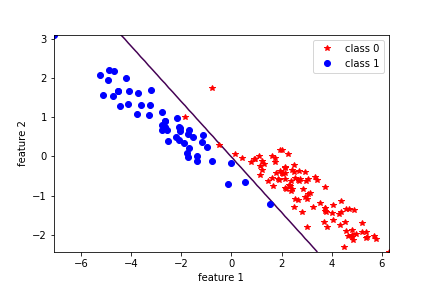
\includegraphics[scale=0.7]{figures/fig_fisher_lda_datasetA.png}
	\caption{\small{Data from the dataset A represented as a point cloud in $\mathbb{R}^2$ and the line defined by the equation $p(y=1\mid x)$ using the Fisher LDA learning algorithm.}}
	\label{fig:lda_datasetA}
\end{figure}
\begin{figure}[ht]
	\center
	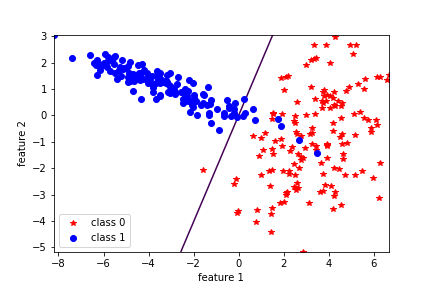
\includegraphics[scale=0.7]{figures/fig_fisher_lda_datasetB.png}
	\caption{\small{Data from the dataset B represented as a point cloud in $\mathbb{R}^2$ and the line defined by the equation $p(y=1\mid x)$ using the Fisher LDA learning algorithm.}}
	\label{fig:lda_datasetB}
\end{figure}
\begin{figure}[ht]
	\center
	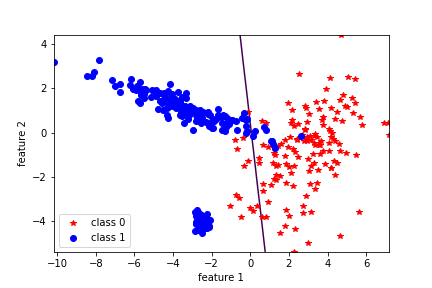
\includegraphics[scale=0.7]{figures/fig_fisher_lda_datasetC.png}
	\caption{\small{Data from the dataset C represented as a point cloud in $\mathbb{R}^2$ and the line defined by the equation $p(y=1\mid x)$ using the Fisher LDA learning algorithm.}}
	\label{fig:lda_datasetC}
\end{figure}

\end{description}

\clearpage

\section{Logistic regression}\label{sec:logistic}

\begin{description}

\item [(a)] The numerical values of the learnt parameters for each training set are given here. For dataset A, we have :

\begin{equation}
w = \begin{bmatrix} -5.54892822 \\ -9.01885324 \end{bmatrix} \qquad b = -0.717570
\end{equation}

For dataset B, the learnt parameters are the following :

\begin{equation}
w = \begin{bmatrix} -0.70215844 \\ 0.36482568 \end{bmatrix} \qquad b = 0.154877
\end{equation}

Finally, for dataset C, we have :

\begin{equation}
w = \begin{bmatrix} -1.69277685 \\ 0.37903323 \end{bmatrix} \qquad b = 0.569075
\end{equation}

\item [(b)] Here are presented the data and the line defined by the equation $p(y=1\mid x)$ for the three training datasets.

\begin{figure}[ht]
	\center
	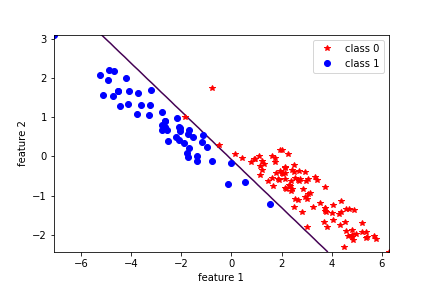
\includegraphics[scale=0.7]{figures/fig_logistic_regression_datasetA.png}
	\caption{\small{Data from the dataset A represented as a point cloud in $\mathbb{R}^2$ and the line defined by the equation $p(y=1\mid x)$ using the logistic regression learning algorithm.}}
	\label{fig:logit_datasetA}
\end{figure}
\begin{figure}[ht]
	\center
	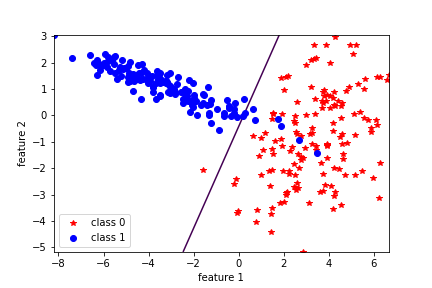
\includegraphics[scale=0.7]{figures/fig_logistic_regression_datasetB.png}
	\caption{\small{Data from the dataset B represented as a point cloud in $\mathbb{R}^2$ and the line defined by the equation $p(y=1\mid x)$ using the logistic regression learning algorithm.}}
	\label{fig:logit_datasetB}
\end{figure}
\begin{figure}[ht]
	\center
	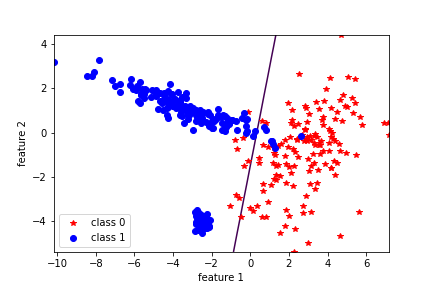
\includegraphics[scale=0.7]{figures/fig_logistic_regression_datasetC.png}
	\caption{\small{Data from the dataset C represented as a point cloud in $\mathbb{R}^2$ and the line defined by the equation $p(y=1\mid x)$ using the logistic regression learning algorithm.}}
	\label{fig:logit_datasetC}
\end{figure}

\end{description}

\clearpage

\section{Linear regression}\label{sec:linear}

\begin{description}

\item [(a)] The numerical values of the learnt parameters for each training set are given here. For dataset A, we have :

\begin{equation}
w = \begin{bmatrix} -0.2640075 \\ -0.37259311 \end{bmatrix} \qquad b = 0.492292
\end{equation}

For dataset B, the learnt parameters are the following :

\begin{equation}
w = \begin{bmatrix} -0.10424575 \\ 0.05179118 \end{bmatrix} \qquad b = 0.500050
\end{equation}

Finally, for dataset C, we have :

\begin{equation}
w = \begin{bmatrix} -0.12769333 \\ -0.01700142 \end{bmatrix} \qquad b = 0.508400
\end{equation}

\item [(b)] Here are presented the data and the line defined by the equation $p(y=1\mid x)$ for the three training datasets.

\begin{figure}[ht]
	\center
	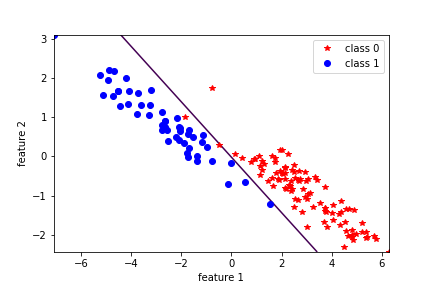
\includegraphics[scale=0.7]{figures/fig_linear_regression_datasetA.png}
	\caption{\small{Data from the dataset A represented as a point cloud in $\mathbb{R}^2$ and the line defined by the equation $f(x) = 0.5$ using the linear regression learning algorithm.}}
	\label{fig:lin_datasetA}
\end{figure}
\begin{figure}[ht]
	\center
	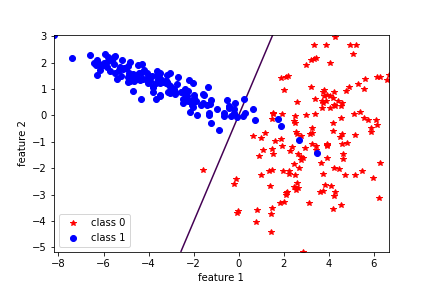
\includegraphics[scale=0.7]{figures/fig_linear_regression_datasetB.png}
	\caption{\small{Data from the dataset B represented as a point cloud in $\mathbb{R}^2$ and the line defined by the equation $f(x) = 0.5$ using the linear regression learning algorithm.}}
	\label{fig:lin_datasetB}
\end{figure}
\begin{figure}[ht]
	\center
	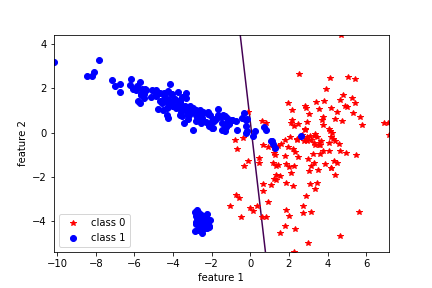
\includegraphics[scale=0.7]{figures/fig_linear_regression_datasetC.png}
	\caption{\small{Data from the dataset C represented as a point cloud in $\mathbb{R}^2$ and the line defined by the equation $f(x) = 0.5$ using the linear regression learning algorithm.}}
	\label{fig:lin_datasetC}
\end{figure}

\end{description}

\clearpage

\section{Error and performance of the models}\label{sec:error}

\begin{description}

\item [(a)] The misclassification error on the training set and the test set for each model is presented in table \ref{tab:error} below.

\begin{table}[ht]
\centering
 \begin{tabular}{| c || c | c | c | c | c | c |}
    \hline
     &
      \multicolumn{2}{c}{Dataset A} &
      \multicolumn{2}{c}{Dataset B} &
      \multicolumn{2}{c|}{Dataset C} \\
    & Train & Test & Train & Test & Train & Test \\
    \hline
    Fisher LDA & 1.33\% & 2.00\% & 3.00\% & 4.15\% & 5.50\% & 4.23\% \\
    \hline
    Logistic regression & 0.67\% & 2.47\% & 2.67\% & 4.00\% & 4.00\% & 2.63\% \\
    \hline
    Linear regression & 1.33\% & 2.13\% & 3.33\% & 4.20\% & 6.25\% & 4.60\% \\
    \hline
  \end{tabular}
\caption{\label{tab:error}\small{Misclassification error on training sets and test sets for the different learning algorithms.}}
\end{table}

\item [(b)] The misclassification error obtained for the various learning algorithms are pretty similar for a given dataset. First of all, we see that the misclassification error is lower for the training dataset than for the test dataset for datasets A and B, but not for dataset C for all learning algorithms that were used. This may be due to the fact that dataset C had a more complicated data distribution, which could not be easily separated by a simple linear boundary. For datasets A and B, the learnt parameters were far more precise for separating the training dataset, but could not generalize as well on data it had never seen before, which is why the misclassification error on the test set is higher than the one on the training set for those datasets.

One important thing to notice is that the logistic regression, which is based on a iterative second order gradient descent method, tends to overfit the data for dataset A. We can clearly see that the misclassification error is really low on the training set while it is much more high for the test set. In fact, if a maximum of iterations hadn't been implemented, the optimization would have continued for much longer, which would have given a worse misclassification error on the test set while giving a slightly better one for the training set. This situation was unique to this learning algorithm since the other methods were not based on an iterative optimization. However, the logistic regression model did fairly well for the other datasets, obtaining the best results for both of them in all the test sets and training sets.

Both the Fisher LDA model and the linear regression model yielded similar results for all three datasets on which they were trained although those results were not better than the ones obtained by the logistic regression model for datasets B and C.

\end{description}

\clearpage

\section{QDA model}\label{sec:qda}

\begin{description}

\item [(a)] The numerical values for the learnt parameters using the QDA model are given below. For dataset A, we have :

\begin{equation}
\Pi = 0.33 \quad \mu_0 = \begin{bmatrix}2.89970947 \\ -0.893874 \end{bmatrix} \quad \mu_1 = \begin{bmatrix}-2.69232004 \\ 0.866042 \end{bmatrix}
\end{equation}
\begin{equation*}
\Sigma_0 = \begin{bmatrix} 2.31065259 & -1.04748461 \\ -1.04748461 & 0.57578403 \end{bmatrix} \quad \Sigma_1 = \begin{bmatrix} 2.70442172 & -1.3008515 \\ -1.3008515 & 0.68969588 \end{bmatrix} 
\end{equation*}

For dataset B, the numerical values obtained are :

\begin{equation}
\Pi = 0.5 \quad \mu_0 = \begin{bmatrix}3.34068896 \\ -0.83546333 \end{bmatrix} \quad \mu_1 = \begin{bmatrix}-3.21670734 \\ 1.08306733 \end{bmatrix}
\end{equation}
\begin{equation*}
\Sigma_0 = \begin{bmatrix} 2.79304824 & 1.0642112 \\ 1.0642112 & 2.96007891 \end{bmatrix} \quad \Sigma_1 = \begin{bmatrix}4.15361075 & -1.33454097 \\ -1.33454097 & 0.51607059 \end{bmatrix} 
\end{equation*}

Finally, for dataset C, we have:

\begin{equation}
\Pi = 0.625 \quad \mu_0 = \begin{bmatrix}2.79304824 \\ -0.83838667 \end{bmatrix} \quad \mu_1 = \begin{bmatrix}-2.94232885 \\ -0.9578284 \end{bmatrix}
\end{equation}
\begin{equation*}
\Sigma_0 = \begin{bmatrix} 2.89913927 & 1.24581553 \\ 1.24581553 & 2.92475448 \end{bmatrix} \quad \Sigma_1 = \begin{bmatrix}2.86914403 & -1.76197061 \\ -1.76197061 & 6.56438626 \end{bmatrix} 
\end{equation*}

\item [(b)] The graphical representations of the data as well as the conic defined by $p(y=1\mid x) = 0.5$ are presented below for each dataset.

\begin{figure}[ht]
	\center
	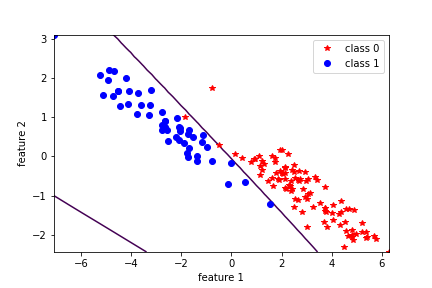
\includegraphics[scale=0.7]{figures/fig_qda_datasetA.png}
	\caption{\small{Data from the dataset A represented as a point cloud in $\mathbb{R}^2$ and the line defined by the equation $p(y=1\mid x) = 0.5$ using the QDA learning algorithm.}}
	\label{fig:qda_datasetA}
\end{figure}
\begin{figure}[ht]
	\center
	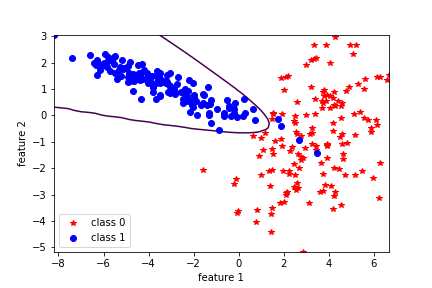
\includegraphics[scale=0.7]{figures/fig_qda_datasetB.png}
	\caption{\small{Data from the dataset B represented as a point cloud in $\mathbb{R}^2$ and the line defined by the equation $p(y=1\mid x) = 0.5$ using the QDA learning algorithm.}}
	\label{fig:qda_datasetB}
\end{figure}
\begin{figure}[ht]
	\center
	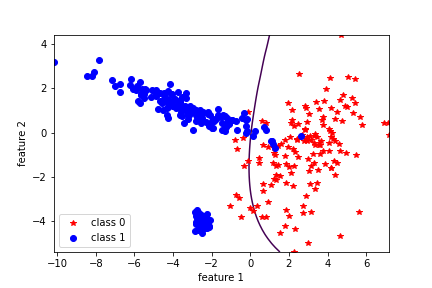
\includegraphics[scale=0.7]{figures/fig_qda_datasetC.png}
	\caption{\small{Data from the dataset C represented as a point cloud in $\mathbb{R}^2$ and the line defined by the equation $p(y=1\mid x) = 0.5$ using the QDA learning algorithm.}}
	\label{fig:qda_datasetC}
\end{figure}

\clearpage
\item [(c)] The misclassification error for QDA all datasets for both train and test data is presented in the table below.

\begin{table}[ht]
\centering
 \begin{tabular}{| c || c | c | c | c | c | c |}
    \hline
     &
      \multicolumn{2}{c}{Dataset A} &
      \multicolumn{2}{c}{Dataset B} &
      \multicolumn{2}{c|}{Dataset C} \\
    & Train & Test & Train & Test & Train & Test \\
    \hline
    QDA & 0.67\% & 2.00\% & 1.33\% & 2.00\% & 5.25\% & 3.83\% \\
    \hline
  \end{tabular}
\caption{\label{tab:error_qda}\small{Misclassification error on training sets and test sets for the QDA model.}}
\end{table}

\item [(d)] We see right away that this model is more flexible, allowing us to classify the data more freely than the previous models. In other words, the capacity of the QDA model is greater. The misclassification error obtained for all three datasets is better or equal to the errors obtained with the other models except for the test set of dataset C using logistic regression. The score obtained for the classification of dataset B is far better than any misclassification error obtained with the other models. This was easily predictable since we know that the data from this dataset is distributed from two normal distributions with different mean and covariance matrices, which is precisely the situation for which the QDA model is designed to model. It also does really well on dataset A, which was predictable since it is the case where the data was distributed following two normal distributions with different mean and same covariance matrix. The QDA model can certainly handle this situation with no problem at all. The last situation was the most difficult to model for the learning algorithm, as it was previously with the other models.

\end{description}

\end{document}